\chapter{The Futhark \csharp{} backend}

\begin{figure}[h]
  \centering
  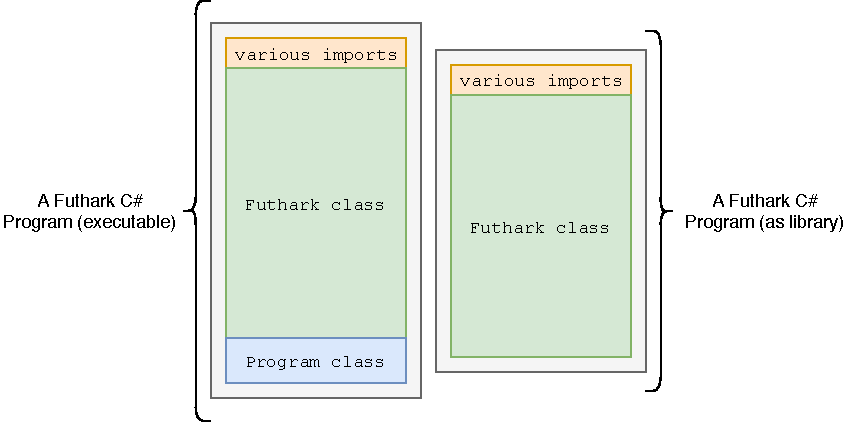
\includegraphics[scale=0.85]{chapters/figs/csharp/futharkcs_wide.pdf}
  \caption{The two possible types Futhark \csharp{} programs}
  \label{fig:futharkcsclasses}
\end{figure}

To be able to use Futhark with \fsharp{} programs, it was necessary to compile
Futhark programs to a language that \fsharp{} could work with.
Although the difference between running a compiled Futhark C- and \csharp{}
executable from the command line is negliable, a Futhark \csharp{} backend would
allow .NET projects to use Futhark libraries natively, instead of running their
Futhark calculations through seperate C or Python modules.

Because \fsharp{} has almost frictionless interoperability with \csharp{}, and \csharp{}s
imperative constructs are very close to the intermediate code that Futhark
generates for it's code generation, it was an easy decision to implement a
\csharp{} generating backend for Futhark, to accompany the already existing C-
and Python backends.

A Futhark backend must be able to do two different programs from a given Futhark
program:

First, it must be able to generate standalone executables which can take input data from the \texttt{stdin} stream, and send
the results to the \texttt{stdout} stream. Although a Futhark C, -Python or
\csharp{} executable should have equivalent functionality, their performance may
vary, and the users may alter between the versions depending on which platforms
that are available on their systems.

Second, and more interesting, it must be able to generate single file libraries
which can then be imported and used in other C, Python or \csharp{} projects, in
the same manner as any other library.

\begin{figure}[h]
  \centering
    \begin{lstlisting}[language=Futhark]
      let main (xs : []i32) : []i32 = map (+2) xs
    \end{lstlisting}
  \caption{A very small Futhark program \texttt{map2.fut}}
  \label{fig:smallfut}
\end{figure}
In example, if we compile the Futhark program in figure \ref{fig:smallfut} as a
Python library, we will be able to use it in a Python program, as showed in figure \ref{fig:smallpython}.
Likewise, we would like to be able to do the same thing in a \csharp{} or an
\fsharp{} context.
\begin{figure}[h]
  \centering
    \begin{lstlisting}[language=python]
      import numpy as np
      from map2 import map2

      xs = np.array([1,2,3])
      map2object = map2()
      xs_res = map2object.map2(xs)
      print xs_res # prints [3,4,5]
    \end{lstlisting}
  \caption{A very small Python program}
  \label{fig:smallpython}
\end{figure}

\subsection*{The anatomy of a Futhark \csharp{} program}
In figure \ref{fig:futharkcsclasses}, we see the two different ways we can
compile a Futhark program to \csharp{}. They're largely the same, except for
that the executable Futhark program must have a \texttt{Program} class with a
\texttt{Main} method defined, so that there is an entrypoint defined for the
compiled executable. Furthermore, the Futhark class in the executable version
contains an entry function which chooses what Futhark function to run (in cases
where the Futhark program has more than one entry function defined.) 

The Program class itself (as seen in figure \ref{fig:programclass}) is not especially
interesting, and does only contain a main method which initialises the Futhark
class, and calls the entry function inside the Futhark class.
For both Futhark programs, the top consists of the various imports needed for
the program.

\begin{figure}[h]
  \centering
  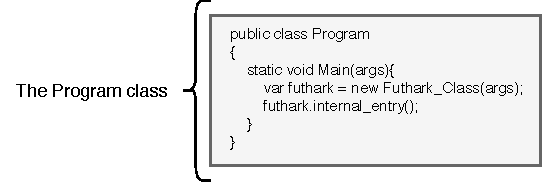
\includegraphics{chapters/figs/csharp/program_class.pdf}
  \caption{The \fshark{} compilation pipeline}
  \label{fig:programclass}
\end{figure}

This leaves us with the Futhark class itself.
Figure \ref{fig:futharkclass} shows the different parts that make up the
generated Futhark \csharp{} class. In the following sections we will walk
through the individual parts.

\begin{figure}[h]
  \centering
  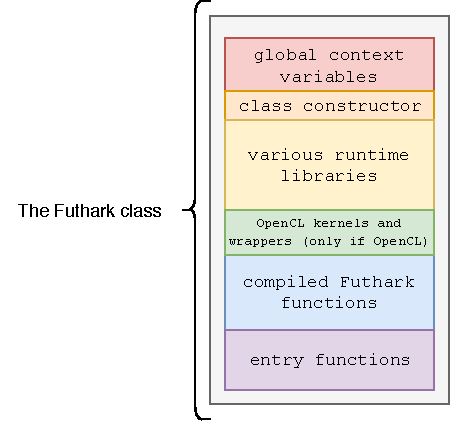
\includegraphics{chapters/figs/csharp/futhark_class.pdf}
  \caption{The layout of the \csharp{} Futhark class}
  \label{fig:futharkclass}
\end{figure}

\subsection*{Global context variables}
\label{globalcontextvariables}
Compiled Futhark programs need to keep track of several variables.
Both normal and OpenCL-enabled Futhark \csharp{} programs can take several
options when they're launched from the command line. In example,
\texttt{num\_runs} tells the Futhark runtime how many times the chosen entry
function should be executed, and the variable \texttt{runtime\_file} tells the
Futhark runtime where it should write timing information to, for example for
benchmarking purposes.

Instead of passing an argument array along throughout all the functions in the
Futhark class, like we usually would if we were writing purely functional
programs, we instead set these arguments as class variables at class
initialization, so we can refer to them everywhere throughout the rest of the class.

For non-OpenCL programs, the variables are exclusively for benchmarking and
debugging purposes. For OpenCL programs however, the global variables are vital
for the program's execution.
In an OpenCL program, the Futhark class must keep track of two extra
variables.

The struct \texttt{futhark\_context ctx} is the struct that contains the global
state of the current program's execution. Contained in the global state there is
the current list of unused but allocated OpenCL buffers on the device, kernel
handles for all the OpenCL kernels used in the Futhark program, and a counter
for the total running time of the program.
There is even another context contained in the \texttt{futhark\_context}, namely
the \texttt{opencl\_context}, which contains the current state of the device,
and also information about it's platform, it's queue and so forth.

The struct \texttt{futhark\_context\_config cfg} is similar to the
\texttt{futhark\_context}, but is only used for constructing the actual
\texttt{futhark\_context}.

\subsection*{The class constructor}
The class constructor is necessary to setup the global variables needed
throughout the Futhark class. When the Futhark program is compiled as an
executable, the command line arguments are passed to the class constructor by
the \texttt{Program} class. If the Futhark program is compiled as a library, the
programmer can pass a string array of arguments to this constructor manually.

Besides setting class variables, OpenCL-enabled versions will initialize (and
set) first the \texttt{futhark\_context\_config cfg} variable, and afterwards
the \texttt{futhark\_context} itself.

\subsection*{The various runtime libraries}
The runtime libraries are a set of seperate \csharp{} files that are written and
distributed through the Futhark compiler. When a Futhark program is compiled,
these library files are concatenated and embedded directly into the rest of the
generated code. They contain functionality which the generated Futhark programs
depend on.
The runtime libraries are the following:
\begin{description}
\item[\texttt{memory.cs}] \hfill\\
  As Futhark's stores all array values (no matter the dimensionality) as a flat one-dimensional byte arrays (with an accompanying
  array of 64-integers which denote the dimensions of the flat array), it was
  necessary to define a set of functions to interact with these byte arrays.
  I.e., \texttt{memory.cs} contains the \texttt{writeScalarArray} functions,
  which writes a scalar value to a byte array. The function is overloaded so it
  works with scalars of any integer or floating point primitive. See figure
  \ref{fig:writeScalarArray} for an example:

\begin{figure}[h]
\centering
\begin{minted}[fontsize=\small]{csharp}
void writeScalarArray(byte[] dest, int offset, double value)
{
    unsafe
    {
        fixed (byte* dest_ptr = &dest[offset])
        {
            *(double*) dest_ptr = value;
        }
    }
}
\end{minted}
\caption{\texttt{writeScalarArray} writes a value at the specified offset in
some byte array.}
\label{fig:writeScalarArray}
\end{figure}

\item[\texttt{scalar.cs}] \hfill\\
  This library contains all the scalar functions necessary for Futhark \csharp{}
  programs.
  In Futhark, arithmetic operators are defined for integers and floats of all
  sizes, and bitwise operators are defined for all integers.
  However, this is not the case in \csharp{}, where many arithmetic operators
  are only defined for 32- and 64 bit integers.
  
  If these operators are used with 8- or 16 bit operands, the operands are
  implicitly casted to 32 bit integers at compile time, which also means that
  the final result of the operation is a 32 bit integer, which doesn't has the
  right type.

  Therefore, wrapper functions must be defined for even the simplest arithmetic
  functions. I.e., integer addition in \csharp{} Futhark is actually four different
  functions:
\begin{minted}[fontsize=\small]{csharp}
static sbyte add8(sbyte x, sbyte y){ return Convert.ToSByte(x + y); }
static short add16(short x, short y){ return Convert.ToInt16(x + y); }
static int add32(int x, int y){ return x + y; }
static long add64(long x, long y){ return x + y; }
\end{minted}

  Besides, \texttt{scalar.cs} also contains the \csharp{} definitions for the various
  mathematical functions from Futhark's \texttt{math.fut}library, such as \texttt{exp},
  \texttt{sin} and \texttt{cos}.

\item[\texttt{reader.cs}] \hfill\\
  The reader contains the entire functionality for recieving function parameters
  through \texttt{stdin}. The reader reads scalars of any of the
  Futhark-supported primitives, and also arrays and multidimensional arrays of
  scalars.
  The reader also supports reading streams of binary data.
  It is only necessary for Futhark executables.
\item[\texttt{opencl.cs}] \hfill\\
  MAYBE WRITE ALL OF THIS ALSO? ALRIGHT THANKS
\end{description}

\subsection*{The compiled Futhark functions}
  The compiled Futhark functions are the Futhark Intermediate Code functions,
  expressed in the target language, and corresponds to the entry functions found
  in the entry functions-section of the Futhark class.
  Only the Futhark \texttt{entry} functions are compiled to individual functions, and
  remaining helper functions are inlined here.

  In OpenCL programs, all array functions and SOAC calls are compiled as
  individual (or fused) OpenCL kernels. Therefore, the compiled Futhark
  functions in these programs consists of mainly some scalar operations and
  memory allocations, and calls to Futhark-generated kernel wrapper functions.
  
  In non-OpenCL programs, the array functions and SOAC calls are not stored in
  seperate wrapper functions, but inlined in the Futhark functions.

\subsection*{OpenCL kernels and wrappers}
  If the Futhark program is compiled for OpenCL, all array handling function- and
  SOAC calls are compiled as OpenCL kernels. This part of the Futhark class
  has two parts:
  \begin{enumerate}
  \item The string (actually a single string in an array) \texttt{opencl\_prog}, which contains the entire
  Futhark-generated OpenCL source code for the Futhark program in question.
  This source code contains all the OpenCL kernels for the program, and is
  passed to the OpenCL device, compiled and loaded, when the Futhark class is
  initialized. Handles to the individual kernels are then stored in the \texttt{futhark\_context}.

  \item For each kernel in the \texttt{opencl\_prog}, the Futhark compiler
    generates a kernel wrapper function. These wrapper functions takes the
    kernel arguments (such as scalar values, array values and indexes) as input,
    and performs all the OpenCL specific work necessary for the actual kernel
    launch; in example setting the kernel arguments on the device, and copying
    data back and forth between host and device buffers.
  \end{enumerate}

\subsection*{Entry functions}
Futhark's internal representation of array values are one dimensional byte
arrays (which can represent arrays of any type and dimensionality), and an
accompanying list of integers denoting the lengths of the array's dimensions.
However, Futhark does not expect it's users to pass this form of arrays as
function arguments, which is why each Futhark \texttt{entry} function has a
corresponding entry function in the final compiled code.
\\\\
To discern between Futhark functions and entry functions, the Futhark function's
name is prefixed with ``\texttt{futhark\_}'', as in for example
``\texttt{futhark\_foo}''.
Depending on whether the Futhark program is compiled as an executable or a
library, the entry function itself is then named ``\texttt{entry\_foo}'' or
just ``\texttt{foo}''.

For executables, ``\texttt{entry\_foo}'' is a function that doesn't take any
arguments. Instead, it uses the reader functions from \texttt{reader.cs} to parse the
arguments for ``\texttt{foo}'' from \texttt{stdin}, and passes them to the
Futhark function. For all array values in the arguments, the array values are
converted into Futhark representations of them.
When the Futhark function returns the result, the result is then printed to \texttt{stdout}.

For libraries, the ``\texttt{entry\_}'' prefix is dropped, and the function
just takes care of converting array arguments into and back-from their Futhark
representations.

\clearpage

\section*{The \csharp{} backend, compared to the C- and Python counterparts}

%% DESCRIBE THE DIFFERENCES BETWEEN C# AND THE REST
THE PYTHON BACKEND HAS MUCH FUNCTIONALITY ENCAPSULATED IN PYOPENCL, AND DOESN'T
NEED TO DECLARE VARIABLES BEFORE SETTING THEM
LESS COMPLEX GENERATOR NEEDED AS VARIOUS OPENCL STATEMENTS ARE HANDLED
AUTOMATICALLY BY LIBRARY

C BACKEND MUST BE AWARE OF ALL SIZES AND EVERYTHING AT COMPILE TIME, WHICH MEANS
STATES MUST BE ALLOCATED THROUGH COMPLEX STRUCTS AT COMPILE TIME, AND STRUCTS
MUST BE DEFINED AT COMPILE TIME AS WELL

C ALLOWS NULL POINTERS, CS DOES NOT WHICH MEANS WE NEED PLACEHOLDER VARIABLES

CSHARP GENERATOR IS SOMEWHERE INBETWEEN AS IT IS CAN HANDLE OBJECTS WHICH CAN
CARRY STATE, FURTHERMORE DYNAMIC MEMORY ALLOCATION

% THE DIFFERENCES BETWEEN MEMORY HANDLING IN CS AND CSOPENCL
\section*{Memory management in Futhark \csharp{}}
As Futhark stores array values around in byte arrays, it is relevant to compare
the difference between how the array handling differs between Futhark's C
backend, and this \csharp{} backend.
For OpenCL programs, the memory management of \csharp{} and C is largely the
same, as the OpenCL side of these programs are the same. \csharp{} does after
all just use C bindings for it's OpenCL interactions.

However, for non-OpenCL \csharp{} programs, we have to take \csharp{}'s memory
model into consideration

C implicitly allows unsafe programming. In this case, it means interacting with system
memory by reading and writing arbitrary values from/to arbitrary locations,
designating the values and destinations as whatever type we want.
In figure \ref{fig:futharkcscene}, we see a \texttt{for}-loop that
performs a summing scan on an array of integers.
On line 6, reading from right to left, we are first creating reference to
a location in the byte array \texttt{xs\_mem\_4223}. However, as the reference
is a pointer to a byte in the array, we must recast it as an \texttt{int32\_t} pointer.
After we do this, we can finally derefer the pointer to retrieve a four byte
integer from the byte array.

We add the retrieved integer to our accumulating variable
\texttt{scanacc\_4187}, before we cast a reference in our destination byte array
as an integer pointer, and store the result there.

\begin{figure}
\centering
\begin{minted}[linenos, fontsize=\small]{c}
memblock mem_4226;
memblock_alloc(&mem_4226, bytes_4224);
int32_t scanacc_4187 = 0;

for (int32_t i_4189 = 0; i_4189 < sizze_4135; i_4189++) {
    int32_t x_4147 = *(int32_t *) &xs_mem_4223[i_4189 * 4];
    
    scanacc_4187 += x_4147;

    *(int32_t *) &mem_4226[i_4189 * 4] = scanacc_4187;
}
\end{minted}
\caption{A short snippet from a Futhark C program}
\label{fig:futharkcscene}
\end{figure}

WHY IS THIS NOT ALLOWED?

DESCRIBE TWO DIFFERENT WAYS OF DOING IT ANYHOW
1) MARSHAL
2) unsafe and fixed

what was chosen and why

% WHY THIS DESIGN

% benchmarks are available in benchmarking chapter
%% FOR CS-OPENCL, PERFORMANCE IS COMPARABLE TO C-OPENCL
%% FOR CS, PERFORMANCE IS VASTLY INFERIOR TO TO C
%%% WHY IS THAT???????????

\section*{The \csharp{} / OpenCL interaction}
OpenCL interaction is not a part of the .NET standard library, but several
libraries do exist for .NET/OpenCL interactions. For this thesis, I researched a
selection of these libraries, to determine which one that would fit the best for
my purposes.
As Futhark depends on being able to interface with the OpenCL platform directly,
it was necessary to find an OpenCL library for .NET which had direct bindings to
the OpenCL developer library.

The .NET libraries I took into consideration was \texttt{NOpenCL}, \texttt{OpenCL.NET} and \texttt{Cloo}.
All three libraries have been designed to aide OpenCL usage in \csharp{}
programs, by simplifying OpenCL calls behind methods GØR BEDRE.
\\
\\
\texttt{NOpenCL} was the first candidate for the \csharp{} backend, and had
several advantages to the other two: As per February 2018, it had been updated
within the last year, and was therefore the least deprecated library. Second,
the \texttt{NOpenCL} repository on Github contains both unit tests and
example programs.

However, \texttt{NOpenCL} is also tailored for Windows use, and therefore not a
good fit for Futhark, as Futhark is available on both Windows, Linux and Mac OS.
Furthermore, the library is not available through the NuGet
package manager, and the OpenCL API calls are needlessly complex to work with
through the library.
\\
\\
\texttt{OpenCL.NET} also has a test suite, is available through NuGet, and is
used as the backend for other libraries, such as the \fsharp{} GPU library
\texttt{Brahma.FSharp}\ref{relatedwork:brahma}.

However, this library hardcoded to work on a in a Windows context, and has not been
updated for more than five years.
\\
\\
This leaves us with \texttt{Cloo}. \texttt{Cloo} is usable on all three
platforms, and it is available on NuGet. Furthermore, as opposed to the other two libraries, the
Cloo library contains a class with static functions that does nothing but
passing arguments on to the OpenCL library, using \csharp{}s \texttt{DllImport}
attribute. It is immediately possible to skip most of \texttt{Cloo}s features,
and just use the library for it's OpenCL bindings.

Even then, \texttt{Cloo} has not been updated within the last five years, and
probably won't be in the future either.
\\
\\
Given these three candidates, I chose to work with \texttt{Cloo}: It was the
only one that had the necessary OpenCL bindings readily available, and the only
one that was platform agnostic.

\subsection*{Writing a custom OpenCL bindings library}
Though \texttt{Cloo} is a good fit for Futhark \csharp{}, it is also slightly
risky to depend on a five year old unmaintained library in a modern project.
Therefore, it could be a good idea to write a smaller library similar to
\texttt{Cloo}, specifically for Futhark - or maybe even just include it with
Futhark as one of the \csharp{} runtime libraries. 

%%% Local Variables:
%%% mode: latex
%%% TeX-master: "../thesis"
%%% End: